\chapter{Path-polarization-entangled photons}
\labelChapter{path_polarization_entangled_photons}

\begin{epigram}{\textit{Peter Shor, Quantum Poetry Tweet Collection}}
	\enquote{
		Am I a wave? Am I a particle? Am I analog or digital?\newline
		The answer surely must be both or none.\newline
		My laws say quarks and clocks alike show interference,\newline
		That if you watch a state, it never changes,\newline
		That two entangled systems act as one.} 
\end{epigram}

\section{Introduction: Multi-degree of freedom entanglement}
\lettrine[lines=3]{T}{he} preceding chapter describes the generation of a two-photon two-qubit polarization-entangled state \via the process of \acs{SPDC} with type-I phase matching. In this chapter, we endeavor to describe and experimentally realize one possible way to enlarge this two-qubit state to a state of more qubits. From the previous chapter, one can at least get an inkling that the generation of entangled photons by way of \acs{SPDC} is appealing due to its accessibility, in the case of type-I \acs{SPDC}, ease of alignment and relatively high photon counts in comparison to type-II phase matched \acs{SPDC}~\cite{Kwiat_1999}. Thus one could possibly conceive of a way to enlarge the aforesaid two-qubit state \via the same \acs{SPDC} process; a string of successive \acs{SPDC} processes producing a pair of entangled photons at each step, as done in the experiments of Ref.~\cite{Lu_2006,Huang_2011,Wang_2016}. One potential and sizeable obstacle to such methods is decoherence. As briefly alluded to in the previous chapter, unless one incorporates methods to counteract some of the effects of decoherence on \acs{SPDC} sources such as phase-compensation ~\cite{Akselrod_2007,Rangarajan_2009} to improve the brightness of the source, experiments making use of cascaded \acs{SPDC} processes typically suffer from low efficiencies~\footnote{Due to the decoherence mechanisms of \acs{SPDC} source, but also due to inefficiencies of the optics in the experiment, \eg the collection and detection inefficiencies.}

\bigskip
\noindent
Hitherto, we have only considered the polarization \acs{DOF}, however photon pairs generated in this way also possess various forms of entanglement. The phase-matching conditions for \acs{SPDC} give rise to conservation laws for both energy and momenta of the photon pairs, as a result the pairs are entangled in these continuous \acs{DOFS} as well. The experiments of Rarity \etal~\cite{Rarity_1990} and Kwiat \etal~\cite{Kwiat_1993} were few of the first to demonstrate a violation of a Bell-inequality for a continuous \acs{DOFS}, energy (and time) and momentum, respectively. 


\clearpage
\noindent
Relatively recent experiments have given evidence that, the process of \acs{SPDC} conserves the orbital angular momentum~\cite{Mair_2001,Vaziri_2002}; demonstrating the generation and analysis of coherent superposition of \gls{LG} transverse spatial modes, and a violation of a Bell-inequality for qutrits. A theoretical justification for this conservation law was later derived by Franke-Arnold \etal~\cite{Franke-Arnold_2002} from the phase-matching conditions of \acs{SPDC}. For a \acs{LG} mode pump beam carrying the quantum number $l_\text{pump}$~\footnote{Every photon in the beam carries an orbital angular momentum of $\hbar l_\text{pump}$~\cite{Allen_1992}.}, the sum of the corresponding quantum number for signal and idler photons must be the same, \ie $l_\text{signal} + l_\text{idler} = l_\text{pump}$. For a pump beam with $l_\text{pump}=0$, the resultant two-photon \gls{OAM} state will be

\begin{align}
	\ket{\psi}_\text{OAM} &= \alpha_{0,0}\ket{0_1,0_2} + \alpha_{1,-1}\ket{1_1,-1_2} + \alpha_{-1, 1}\ket{-1_1, 1_2} + \ldots\ldots,
\end{align}

\noindent
with the \acs{LG} modes spanning a countably-infinite dimensional Hilbert space, where the kets denote \acs{OAM} states labelled with the indices $l$ and $\alpha$'s denoting their corresponding probability amplitudes; the subscripts $1$ and $2$ represent the signal and idler photons, respectively. 

\bigskip
\noindent
Photons produced \via \acs{SPDC} could result in photons possessing non-classical correlations in degrees of freedom simultaneously, with each \acs{DOF} independently addressable for such measurements. Such multiply-entangled states are called \enquote{hyper-entangled} states, coined by Kwiat~\cite{Kwiat_1997}. For instance, photon pairs produced by a paired \acs{BBO} type-I \acs{SPDC} process, generate a state represented by the product state:

\begin{align}
	\labelEquation{hyper_ent}
			\ket{\Psi}	&\sim (\ket{H_1,H_2} - \ket{V_1,V_2}) \otimes (\ket{-1_1,-1_2} + \ket{1_1,1_2}).
\end{align}

\noindent
For this particular state, each \acs{DOF} is independently addressable and in a well defined state, that is, measurements of observables on either subsystem, whether of polarization or orbital angular momentum, have no bearing on the other subsystem. Formally, a partial trace over the subsystem in either \acs{DOF} leaves the other subsystem unaffected.

\begin{align}
 	\Tr_A(\varrho_{AB}) &= \Tr_A(\varrho_A \otimes \varrho_B), \nonumber \\
 						&= \displaystyle\sum_{i=0}^{3}\ev{\varrho_A}{i}\otimes\varrho_B,\nonumber \\
 						&= \mathds{1}_A \otimes \varrho_B, \nonumber \\
 						&= \varrho_B,
 \end{align}

\noindent
where $\varrho_A = 1/2(\ket{H_1,H_2} - \ket{V_1,V_2})(\bra{H_1,H_2} - \bra{V_1,V_2})$ and $\varrho_B = 1/2(\ket{-1_1,-1_2} + \ket{1_1,1_2})(\bra{-1_1,-1_2} + \bra{1_1,1_2})$, and where $\ket{i}$'s are from the orthonormal basis set $\{\ket{H_1,H_2}, \ket{H_1,V_2}, \ket{V_1,H_2}, \ket{V_1,V_2}\}$ for the polarization subsystem. It is also possible for a \acs{SPDC} source to generate a state of the kind:

\begin{align}
	\labelEquation{hypo_ent}
	\ket{\Psi} \sim (\ket{H_1,H_2,-1_1,-1_2} + \ket{V_1,V_2,1_1,1_2}).
\end{align}

\clearpage
\noindent
Such a state is a little different from the state of~\refEquationOnly
{hyper_ent}. The first obvious difference is this state isn't a product state; the state in either \acs{DOF} can no longer be described separately, we can only collectively describe it by referencing to the state of the other \acs{DOF} \ie the full joint state is non-separable. For such a state (as we've seen elsewhere), a measurement in one \acs{DOF} has a bearing on the other \acs{DOF}. For instance, taking the partial trace over the \acs{OAM}\acs{DOF} yields:

\begin{align}
	\Tr_{CD}(\varrho_{ABCD}) &= \Tr_{AB}(\ket{H_1,H_2,-1_1,-1_2}\bra{H_1,H_2,-1_1,-1_2} \nonumber \\
						&+ \ket{H_1,H_2,-1_1,-1_2}\bra{V_1,V_2,1_1,1_2} \nonumber \\
						&+ \ket{V_1,V_2,1_1,1_2}\bra{V_1,V_2,1_1,1_2}  \nonumber \\
						&+ \ket{V_1,V_2,1_1,1_2}\bra{H_1,H_2,-1_1,-1_2}) \nonumber \\
						&= \ket{H_1,H_2}\bra{H_1,H_2} + \ket{V_1,V_2}\bra{V_1,V_2}.
\end{align}

\noindent
where the partial trace is performed over the basis set $\{\ket{-1_1,-1_2}, \ket{-1_1,1_2}$ $, \ket{1_1,-1_2}, \ket{-1_1,-1_2}\}$. Note that the resultant state is one in which coherences between $\ket{HH}$ and $\ket{VV}$ are completely destroyed; the density matrix of the state has no off-diagonal elements. The said states are called \enquote{hypoentangled states}~\cite{Nathan_PhD}, their defining feature is that they exhibit simultaneous entanglement, but when one of \acs{DOFS} is considered independently, the entanglement in that \acs{DOF} isn't preserved. 

\begin{marginfigure}
	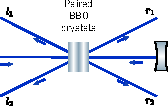
\includegraphics[width=\textwidth]{BF_SPDC.pdf}
	\caption[A \acs{SPDC} source with two concatenated \acs{BBO} crystals stimulated by a pump beam in both directions.]{A \acs{SPDC} source with two concatenated \acs{BBO} crystals stimulated by a pump beam in both directions. The two pairs are emitted in different directions, $l_1, l_2$ and $r_1, r_2$ denoting the four spatial modes.}
	\labelFigure{bf_spdc}
\end{marginfigure}

\bigskip
\noindent
The first demonstration and complete characterization of a hyper entangled photonic quantum system was done by Langford~\cite{Nathan_PhD}, generating and completely characterizing a $144$-dimensional state, simultaneously and independently entangled in polarization, transverse (\acs{OAM}) spatial modes and photon emission times (time-bin encoding). The rarity and novelty of such a demonstration would seem to suggest the experimental difficulity/novelity of realizing photonic states of this kind. Indeed, exerting control over different \acs{DOFS} is not trivial. They often necessitated sophisticated and tricky mode (spatial and/or temporal) matching requirements to implement in practice.

\bigskip
\noindent
The same partly holds true in practice, for similar experiments that generate hyper(hypo) entangled photonics states through polarization and momentum (directions of the emitted photons) \acs{DOFS}. Here, a pump beam stimulates a \acs{SPDC} crystal in both directions resulting in polarization-entangled photon pairs in both directions, which are then appropriately isolated to four optical path modes ($l_1, l_2\text{ and }r_1, r_2$ in~\refFigureOnly{bf_spdc}). If the paired path modes, one mode from the backward photon pair and another from the forward photon pair ($l_1\text{ and }r_1$ and $l_2\text{ and }r_2$) are overlapped temporally (and spatially) on the input ports of a 50:50 beam splitter (see~\refFigureOnly{temporal_delay}), can they can realize a hyperentangled state of the form~\cite{Yang_2005}:

\begin{align}
	\ket{\Psi} \sim (\ket{H_1,V_2} \pm \ket{H_1,V_2})\otimes(\ket{r_2,l_2} \pm \ket{l_1,r_1}),
\end{align}

\begin{marginfigure}
	\raggedright
	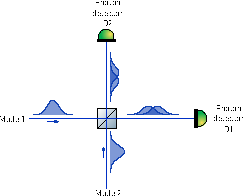
\includegraphics[width=\textwidth]{temporal_delay.pdf}
	\caption[Temporal delay between two spatial modes incident on the input ports of a 50:50 beam splitter.]{Temporal delay between two spatial modes incident on the input ports of a 50:50 beam splitter. The temporal delay leads to temporal indistinguishability, which in an interferometric experiment has a debilitating effect on the observed interference.}
	\labelFigure{temporal_delay}
\end{marginfigure}


\noindent
alternatively if paired path modes belong to the same photon pair ($l_1\text{ and }l_2$ and $r_1\text{ and }r_2$) are similarly overlapped temporally (and spatially) generate the hypoentangled state~\cite{Chen_2007}:

\begin{align}
	\ket{\Psi} \sim (\ket{H_1, H_1} + \ket{V_1,V_2})\ket{l_1,l_2} + (\ket{H_1, H_2} - \ket{V_1,V_2})\ket{r_1,r_2}).
\end{align}


\noindent
In this kind of experimental setup, in addition to the spatial and/or temporal mode matching requirements, the generated state depends on the rate of photon pair emissions in both directions.


\clearpage
\noindent
For the states described above, the aforesaid rates should be equalized. It is known for a \acs{SPDC} source, particularly non-collinear non-degenerate \acs{SPDC}, the resultant (single and joint) spectral profiles, hence the two-photon emission rates and output spatial modes, are dependent on the focus of the pump beam~\cite{Carrasco_2006}. Hence, the experiments in Refs.\cite{Yang_2005, Chen_2007} equalize the emission rates of the two \acs{SPDC} processes (backwards and forwards) using an appropriate arrangement of focusing optics (\ie lens). These added complications compel us to consider an experimental scheme for enlarging our two-photon state from the previous chapter that explicitly avoids them. We consider adopt the experimental scheme of Park \etal~\cite{Park_2007}, which uses a single-photon pair source to realize a polarization-path-entangled state. Hence we describe the experimental design next.

\section{Experimental design}
In this experiment, we extend the experimental setup from the previous chapter to accommodate an additional path qubit. The experimental setup is shown in~\refFigureOnly{experiment_2}; conceptually, this experiment is again simple to describe. The experimental design is similar to the design in the previous chapter (see~\refFigureOnly{experiment_1}) with only one minor addition; in one of the arms, arm $1$ in the figure, the photon beam is incident on a \acs{PBS}, transmitting horizontally-polarized photons and reflecting vertically-polarized photons, which effectively defines our path modes ($l_1\text{ and }r_1$). Our \acs{SPDC} source produces a state close to $(\ket{H_1,H_2} - \ket{V_1,V_2})/\sqrt{2}$, at the dashed line after the action of the \acs{PBS} as shown in~\refFigureOnly{experiment_2} this state becomes:

\begin{align}
	\labelEquation{after_pbs}
	\ket{\Psi_1} = \frac{\ket{H_1, r_1, H_2} - \ket{V_1, l_1, V_2}}{\sqrt{2}}.
\end{align}

\noindent
We designate the polarization and path states of the photon in arm $1$ as qubit $1$ and qubit $2$, respectively and the polarization of the photon in arm $2$ as qubit $3$. Furthermore, relabelling $\ket{H}(\ket{V})$ as $\ket{0}(\ket{1})$, and similarly $\ket{r}(\ket{l})$. The state in~\refEquationOnly{after_pbs} becomes

\begin{align}
	\labelEquation{standard_ghz}
	\ket{\Psi'_1} = \frac{\ket{0, 0, 0} - \ket{1, 1, 1}}{\sqrt{2}} = \frac{\ket{0}^{\otimes 3} - \ket{1}^{\otimes 3}}{\sqrt{2}}.
\end{align}

\noindent
The state in~\refEquationOnly{standard_ghz} is locally equivalent to \acs{GHZ} state~\footnote[][100pt]{Applying the unitary operator ($\mathds{1}_1Z_2\mathds{1}_3$) to $\ket{\Psi}$, we recover the \acs{GHZ} state in its standard form $(\ket{0}^{\otimes 3} + \ket{1}^{\otimes 3})/\sqrt{2}$.}. Similarly, if we apply the unitary operator $U=\mathds{1}Z_2\mathds{1}_3$ to state in~\refEquationOnly{standard_ghz} and proceed to rotate the coordinate system for all our polarization measurements by $\theta=-22.5^{\circ}$ ($\ket{H} \mapsto (\ket{H}+\ket{V})/2, \ket{V} \mapsto (\ket{H} - \ket{V})/\sqrt{2}$), $\ket{\Psi_1}$ becomes:

\begin{align}
	\ket{\Psi_1} = \frac{\ket{+, 0, +} - \ket{-, 1, -}}{\sqrt{2}},
\end{align}

\noindent
where $(\ket{\pm} = \ket{0}\pm\ket{1})/\sqrt{2}$. The above state is a three-qubit linear graph state, which may be generated by applying controlled-$Z$ operations on neighboring qubits ($1-2$ and $2-3$) of the initial resource state $\ket{+}_1\ket{+}_2\ket{+}_3$.

\bigskip
\noindent
The rest of the optics in arm $1$ of the experimental setup are designated for measurement and analysis, consisting of a \acs{MZI}, which combines the two path modes on the output ports of a 50:50 beam splitter. 

\clearpage
\begin{figure*}[t!]
  \centering
  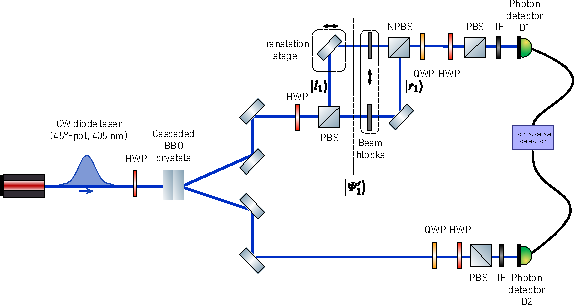
\includegraphics[width=1.0\textwidth]{experiment_2.pdf}%
	\caption[Experimental setup for generation and measurement of a two-photon three-qubit path-polarization-entangled state locally equivalent to a \acs{GHZ} state.]{Experimental setup for generation and measurement of a two-photon three-qubit path-polarization-entangled state locally equivalent to a \acs{GHZ} state.  \gls{HWP}, \gls{QWP}, \gls{BBO}, \gls{PBS}, \gls{NPBS}, translatable mirror,  translatable beam blocks, and \gls{IF}. A photon pair is created whenever a laser pump photon with \SI{405}{nm} wavelength is incident on the paired \acs{BBO} crystals cut for type-I \acs{SPDC}, generating photons at \SI{810}{nm}. One of the photons enters a \acs{MZI} where path modes are made to interfer when combined on , at the dashed line the joint state $\ket{\Psi'_1}$ is locally equivalent to a \acs{GHZ} state. Each photon is guided by a set of mirrors to a \acs{QWP}, \acs{HWP}, and \acs{PBS} which are used to perform polarization measurements of the quantum state. Finally, each photon is sent to an \acs{IF} at \SI{800}{nm} with a bandwidth of \SI{40}{nm} and collected by a \gls{SMF} and sent to a photon detector. Each photon detector produces an electronic signal and sends it to the coincidence counting electronics, which count the signals that arrive simultaneously.}
  \labelFigure{experiment_2}
\end{figure*}


\noindent
One of the path modes is reflected off a mirror on an motorized translation stage (MTS25/M-Z8 - 25 mm (0.98") Motorized Translation Stage with a KDC101 K-Cube Motor Controller), which can used to change the relative phase difference between the two path modes, projecting the path qubit to states on the$x$-$y$ plane of the Bloch sphere (on the equator) with the form:

\begin{align}
	\ket{\varphi} = \frac{\ket{0} + e^{i\varphi}\ket{1}}{\sqrt{2}}.
	\labelEquation{equator_eq}
\end{align}

\noindent
In both paths, there are beam blocks mounted on an electronically-controlled translation stage, which can either block one of the paths or let them both pass. Whenever we block one of the paths, we project out one of the states $(\ket{0}, \ket{1})$ depending on which path is blocked. The combined beam on one of the output ports of the beam splitter is sent to polarization analysis optics and eventually to the photo detector, consisting of a rotatable \acs{QWP} and \acs{HWP}, a \acs{PBS} and an \acs{IF} at \SI{800}{nm} with a \SI{40}{nm} bandwidth. After this stage, the beam goes to a photon detector \via a fibre launch coupled to the detector with a \acs{SMF}. The optical path of arm $1$ is slightly longer than that of arm $2$, for this reason we modify our coincidence counting electronics to add a variable delay to arm $2$ to roughly compensate for the delay on arm $1$ introduced by the \acs{MZI}. Through a bit of tinkering, we find that a delay between \SI{0.5}{ns} to \SI{1.5}{ns} works well enough; our delay electronics operate in increments of \SI{0.5}{ns}, the true delay is probably somewhere in between this range.

\bigskip
\noindent
To match the optical path difference of the two paths to be on the order of the coherence length of the down-conversion photons ($\simeq$ \SI{60}{\micro\meter}) we used a broad spectrum white laser source. The beam from this laser source is guided into the experiment through fibre coupler we previously used to hold the \acs{SMF} taking the beams to the detectors. It is then sent through the \acs{MZI} and collected by another fibre coupler near the crystals coupled with a \acs{SMF} into a spectrometer (Thorlabs CCS200/M with a wavelength range of \SI{200}{nm}-\SI{1000}{nm}). 


\clearpage
\noindent
We can thus resolve the interference fringes in spectra near our collection bandwidth (\SI{800}{nm}$\pm$\SI{40}{nm}) by translating the mirror inside the \acs{MZI} to obtain optimal matching of the path lengths of two arms of the \acs{MZI}. Once the \acs{MZI} is optimized for the coherence length of the down-converted photons, when the two path modes from one of the down-conversion photons combine on the output ports of the 50:50 beam splitter, the state $\ket{\Psi_1}$ of~\refEquationOnly{after_pbs} then becomes:

\begin{align}
	\ket{\Psi_2} = \frac{1}{2}(e^{\varphi_{1}}(\ket{H_1, p_1, H_2} + \ket{H_1, q_1, H_2}) \nonumber \\
	-e^{\varphi_{2}}(\ket{V_1, p_1, V_2} - \ket{V_1, q_1, V_2})),
\end{align}

\noindent
where $p_1, q_2$ are the path modes of the output ports of the beam splitter and $\varphi_{1}, \varphi_{2}$ are the phases acquired by path modes ($l_1$ and $r_1$) by the time they are incident on the beam splitter. Here we adopt the convention $\ket{r_1} \mapsto (\ket{p_1}-\ket{q_1})/\sqrt{2} \text{ and } \ket{l_1} \mapsto (\ket{p_1}+\ket{q_1})/\sqrt{2}$ for the 50:50 beam splitter. After a bit of algebraic deadlifting, the preceding equation becomes:

\begin{align}
	\ket{\Psi_2} = \frac{1}{2}(\ket{p_1}(\ket{H_1, H_2} - e^{i(\varphi_2 - \varphi_1)}\ket{V_1, V_2})) + \nonumber \\
	\ket{q_1}(\ket{H_1, H_2} + e^{i(\varphi_2 - \varphi_1)}\ket{V_1, V_2}))).
\end{align}

\noindent
The mode $q_1$ goes through the polarization analysis optics and eventually to the photon detector yielding:

\begin{align}
	\labelEquation{psi_meas}
	\ket{\Psi_2} = \frac{1}{\sqrt{2}}(\ket{H_1, H_2} + e^{i\varphi}\ket{V_1, V_2}),
\end{align}

\noindent
where $\varphi = \varphi_2 - \varphi_1$. Note that the phase difference between the two path modes influences the state measured by the polarization analysis optics. We can thus infer this phase difference with a similar procedure from our observations in~\refEquationOnly{obs_1} and~\refEquationOnly{obs_2} to optimize the \acs{SPDC} source for a particular Bell state. By inserting a \acs{HWP} in the path mode $r_1$, and setting it at $\theta=45^{\circ}$ ($\ket{H} \leftrightarrow \ket{V}$), ~\refEquationOnly{psi_meas} becomes:

\begin{align}
	\labelEquation{psi_cal}
	\ket{\Psi_2'} &= \frac{1}{\sqrt{2}}(\ket{H_1, H_2} + e^{i\varphi}\ket{H_1, V_2}), \nonumber \\
				  &= \frac{1}{\sqrt{2}}\ket{H_1}(\ket{H_2} + e^{i\varphi}\ket{V_2}).
\end{align}

\noindent
We infer the value $\varphi$ by choosing the appropriate projectors, for instance projecting $P_{HR} = \op{H_1}\otimes\op{L_2}$ on the above state and a bit algebraic deadlifting one obtains the expression for detection probability:

\begin{align}
	&\ev{P_{HR}}{\Psi_2'} = \frac{1}{2} - \frac{1}{2}\sin{\varphi}.
\end{align}

\noindent
Thus moving the translation stage mounted with the mirror, we can minimize the observed coincidence counts which would then correspond to $\varphi = \pi/2$, and maximized coincidence counts correspond to the setting $\varphi = - \pi/2$. The aforementioned values of $\varphi$ project the path qubit in~\refEquationOnly{equator_eq} to $(\ket{0}+i\ket{1})/\sqrt{2}$ and $(\ket{0}-i\ket{1})/\sqrt{2}$, which are the positive and negative eigenvectors of the Pauli matrix $Y$. Any value of $\varphi$ maybe inferred similarly. 


\clearpage
\noindent
Therefore, any equatorial basis measurement of the form:

\begin{align}
	\mathcal{B}(\varphi) = \left\{\frac{\ket{0} + e^{i\varphi}\ket{1}}{\sqrt{2}}, \frac{\ket{0} - e^{i\varphi}\ket{1}}{\sqrt{2}} \right\},
\end{align}

\noindent
can be performed on the path qubit. Together with the $Z$ basis measurements ($\{\ket{0}, \ket{1}\}$), it is possible to perform measurements, measuring each of the eigenvectors of Pauli matrices; which allows us to independently address each of the three qubits for control and measurements of quantum-mechanical correlations of the generated state.

\section{Results}

To get an inkling of how well the \acs{MZI} can contrast between constructive and destructive interference of the two path modes, we measure the fringe visibility for down-conversion photons in following configurations: (i) When only one of the \acs{BBO} crystals, producing the $H$-polarized light cone is stimulated. (ii) When only one of the \acs{BBO} crystals, producing the $V$-polarized light cone. (iii) When both \acs{BBO} crystals are stimulated. For all three configurations, there is a \acs{HWP} at the gate of the interferometer (before the PBS) set to $22.5^{\circ}$ ($\ket{H} \leftrightarrow \ket{D}$), and the half wave-plate in the path mode $r_1$ is set to $\theta=45^{\circ}$, giving the state in~\refEquationOnly{psi_cal} and project out $P_{HD} = \op{H_1}\otimes\op{D_2}$, giving the expression for the detection probability 

\begin{align}
	&\ev{P_{HD}}{\Psi_2'} = \frac{1}{2} + \frac{1}{2}\cos{\varphi},
\end{align}

\noindent
by translating the mirror in the \acs{MZI} in increments of \SI{40}{nm}, we can vary $\varphi$. Typical (normalized) coincidence counts when $\varphi$ is varied for the three aforesaid settings are shown in~\refSubfigureOnly{hh_fringes}, ~\refSubfigureOnly{vv_fringes} and~\refSubfigureOnly{epr_fringes} of ~\refFigureOnly{fringes}, respectively\footnote{The fitting function used for the plots is of the form $a \cos{(b x + c) + d}$. The parameters $a,b,c,d$ were found using Mathematica's \texttt{NonlinearModelFit} function.}. It was worth mentioning that the motor translating the stage can resolve translations down to $\sim$\SI{30}{nm}, however this may come at the price of accuracy. In a sporadic fashion, the motor sometimes translates the mirror slightly less or slightly more than the set step size, hence the plots in the figure above show a few slightly sparse regions. We observe close-to-unity fringe visibilities (calculated from the minima and maxima of the fit) of $0.940$, $0.901$ and $0.921$, respectively. The non-ideal spatial overlap between the two path modes and less-than-unity fidelity of the Bell state prior to the \acs{MZI} may explain the less-than-unity fringe visibility. However, we deem these values sufficient and as indicative that the two path modes are indeed interfering with one another and their optical path difference is within the coherence length of the down-conversion photons. 

\bigskip
\noindent
As we have seen elsewhere, to fully characterize an experimentally generated state, one often needs to perform full \acs{QST}; reconstructing an estimate of the density matrix from which physical quantities of interest may be derived. \acs{QST} for a general three-qubit state would require at least $64$ coincidence measurements. However, if we are only interested in the fidelity of the experimentally generated state and detecting whether the said state possesses genuine multi-particle entanglement around the ideal state we expect to observe, it is possible to circumscribe performing a full tomographic analysis to derive the said quantities, at the cost of generality. 


\clearpage

\begin{figure*}[t!]
    \centering
	\subfloat[\labelFigure{hh_fringes}]
	{
        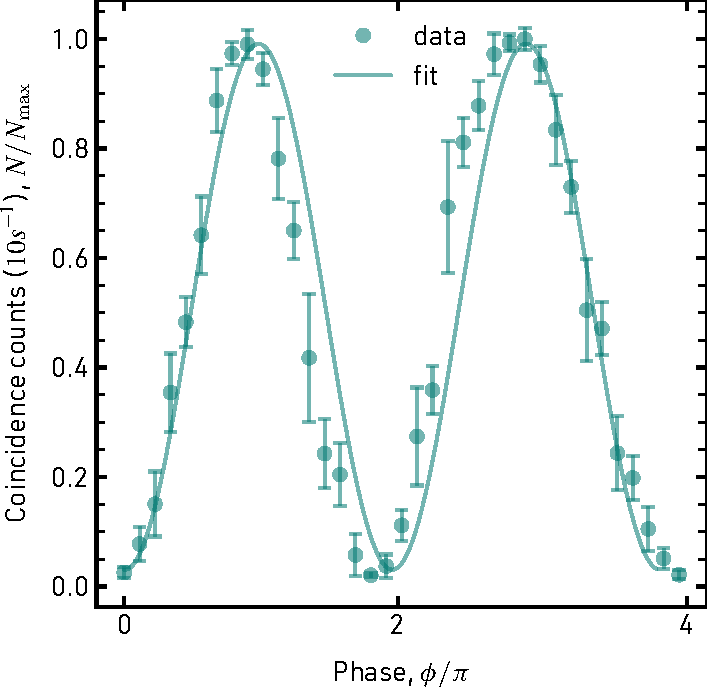
\includegraphics[width=0.33\linewidth]{HH_fringes.pdf}
	}
	\subfloat[\labelFigure{vv_fringes}]
	{
        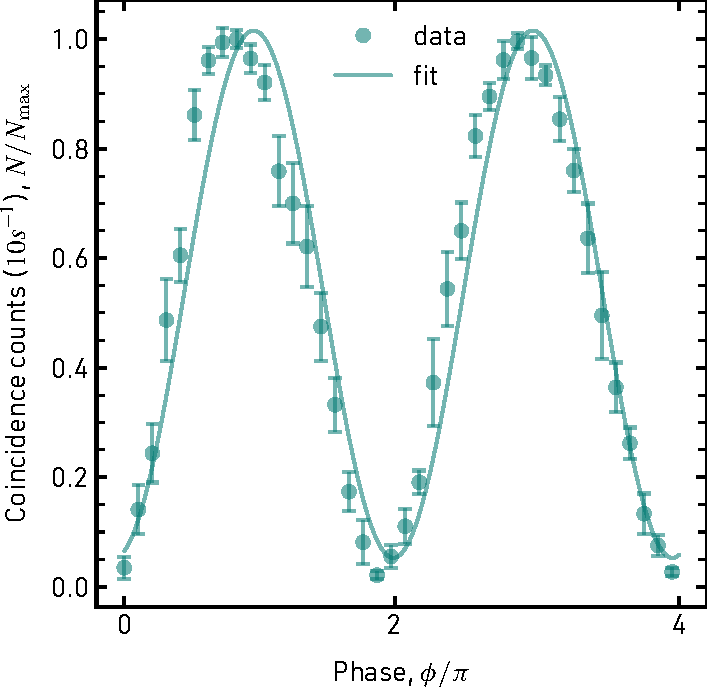
\includegraphics[width=0.33\linewidth]{VV_fringes.pdf}
	}
	\subfloat[\labelFigure{epr_fringes}]
	{
        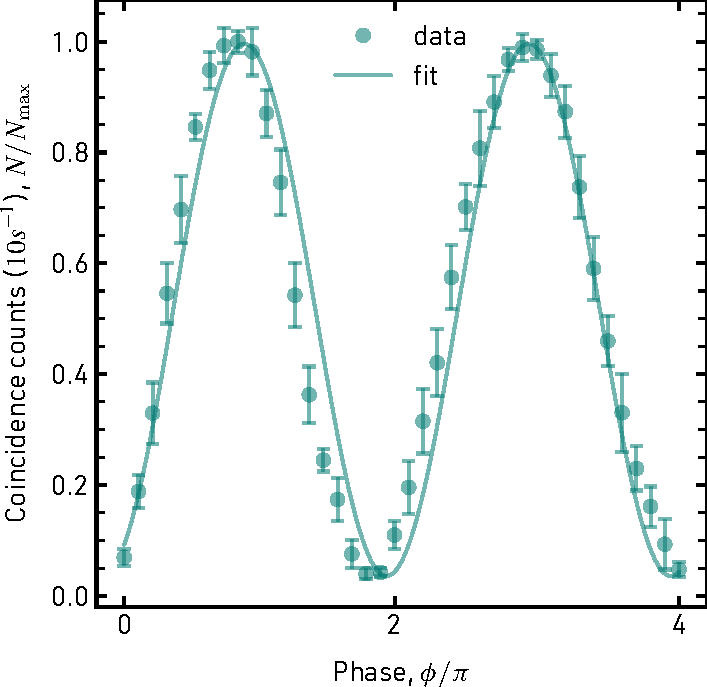
\includegraphics[width=0.33\linewidth]{EPR_fringes.pdf}
	}
	\caption[Photon coincidence counts traversing the \acs{MZI} as a function of the relative phase between the two paths][6pt]{Photon coincidence counts traversing the \acs{MZI} as a function of the relative phase between the two paths in the interferometer: \textbf{(a)} coincidence counts vs. $\phi$ for pairs of only vertically polarized photons \textbf{(b)} Coincidence counts vs $\phi$ for pairs of only horizontally polarized photons \textbf{(c)} Coincidences counts vs $\phi$ for pairs of entangled photons (Bell state). The error bars represent $95\%$ confidence intervals around the mean value (see section~\protect\refSectionOnly{error_bars} of technical~\protect\refAppendixOnly{appendix_A}.}
	\labelFigure{fringes}
\end{figure*}

\noindent
Without directly deriving the density matrix of the experimentally generated state, we can derive an estimate of the fidelity of the generated state from a reduced set of Pauli operator expectation value measurements, in comparison to full \acs{QST}.  Recall that the fidelity between a expected $\varrho$ and measure state $\varsigma$ is given by~\cite{Mike&Ike}:


\begin{align}
	\labelEquation{tr_fid}
	F(\varrho, \varsigma) = \Tr(\sqrt{\sqrt{\varrho}\varsigma\sqrt{\varrho}}^2) = \Tr(\varrho\varsigma).
\end{align}

\noindent
The desired state $\rho$ may be decomposed into a linear combination of $N$-fold products of $\mathds{1}, X, Y, Z$. In the case of a three-qubit \acs{GHZ} state in its standard form, this decomposition is given by:

\begin{align}
	\labelEquation{decomp}
	\varrho &= \frac{1}{8}(\mathds{1}_1\mathds{1}_2\mathds{1}_3 + \mathds{1}_1Z_2Z_3 + X_1X_2X_3 - X_1Y_2Y_3  \nonumber \\
			&\quad- Y_1X_2Y_3 - Y_1Y_2X_3 + Z_1\mathds{1}_2Z_3 + Z_1Z_2\mathds{1}_3).
\end{align}

\noindent
Estimating of the fidelity of our measured state $\varsigma$ amounts to the evaluation of the expectation values\footnote{For any self-adjoint operator $O$, the expectation value of $O$ with respect to the general state $\varsigma$ is given by, $\expval{O} \equiv \Tr(O\varsigma)$} of above operators with respect to the measured state, and summing them up appropriately.  We reduce the number of unique measurements by noting that the expectation value of the terms $\mathds{1}_1Z_2Z_3, Z_1\mathds{1}_2Z_3 \text{ and } Z_1Z_2\mathds{1}_3$ may be derived from the measurement of $Z_1Z_2Z_3$ as their distributions are marginal distributions of $Z_1Z_2Z_3$ when the outcome of the qubit acted on by the identity is not taken into consideration. Similarly, the expectation value of  $\mathds{1}_1\mathds{1}_2\mathds{1}_3$ may derived from any of terms \via marginalization, it is equal to unity in any case\footnote{$\Tr(\mathds{1}_1\mathds{1}_2\mathds{1}_3 \varsigma) = \Tr(\varsigma) = 1$ (normalization condition)}. Thus, we need only evaluate $5$ unique measurements: $X_1X_2X_3, X_1Y_2Y_3,$ $Y_1X_2Y_3,Y_1Y_2X_3, Z_1Z_2Z_3$. Panels~\refSubfigureOnly{xxx},~\refSubfigureOnly{xyy},~\refSubfigureOnly{yxy},~\refSubfigureOnly{yyx} and ~\refSubfigureOnly{zzz} in \refFigureOnly{expvals} show the measurement outcomes ($8$ each) required for the evaluation of the expectation values of the Pauli operators $X_1X_2X_3, X_1Y_2Y_3,$ $Y_1X_2Y_3,Y_1Y_2X_3 \text{ and } Z_1Z_2Z_3$, respectively.  The error bars represent $95\%$ confidence intervals around the mean value (see section ~\refSectionOnly{error_bars} of the technical~\refAppendixOnly{appendix_A}). ~\refTableOnly{expvals} shows the measured expectation values from the measurements in~\refFigureOnly{expvals} of each operator. Evaluating the fidelity using~\refEquationOnly{tr_fid}, and the Pauli decomposition of our expected state in  ~\refEquationOnly{standard_ghz}, we obtain a fidelity of $F_{\varrho}=  0.868\pm0.00996$.

\clearpage

\begin{figure*}[t!]
	\subfloat[\labelFigure{xxx}]
	{
        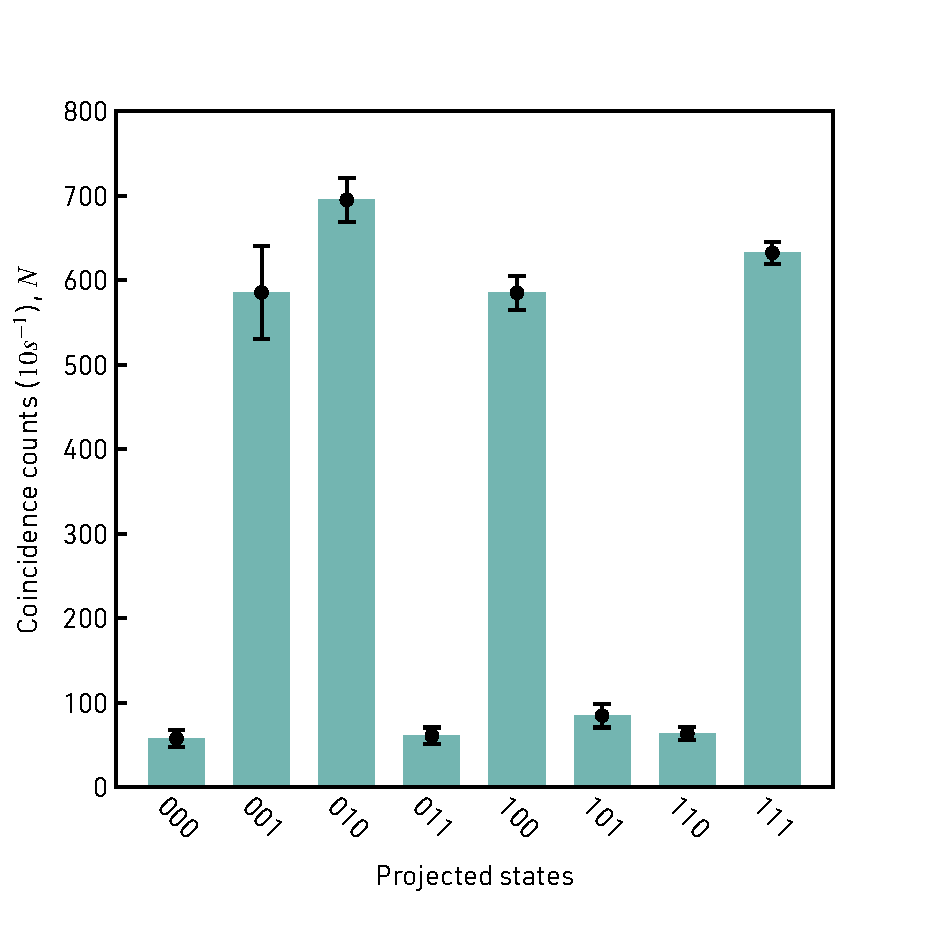
\includegraphics[width=0.33\textwidth]{XXX.pdf}
	}
	\subfloat[\labelFigure{xyy}]
	{
        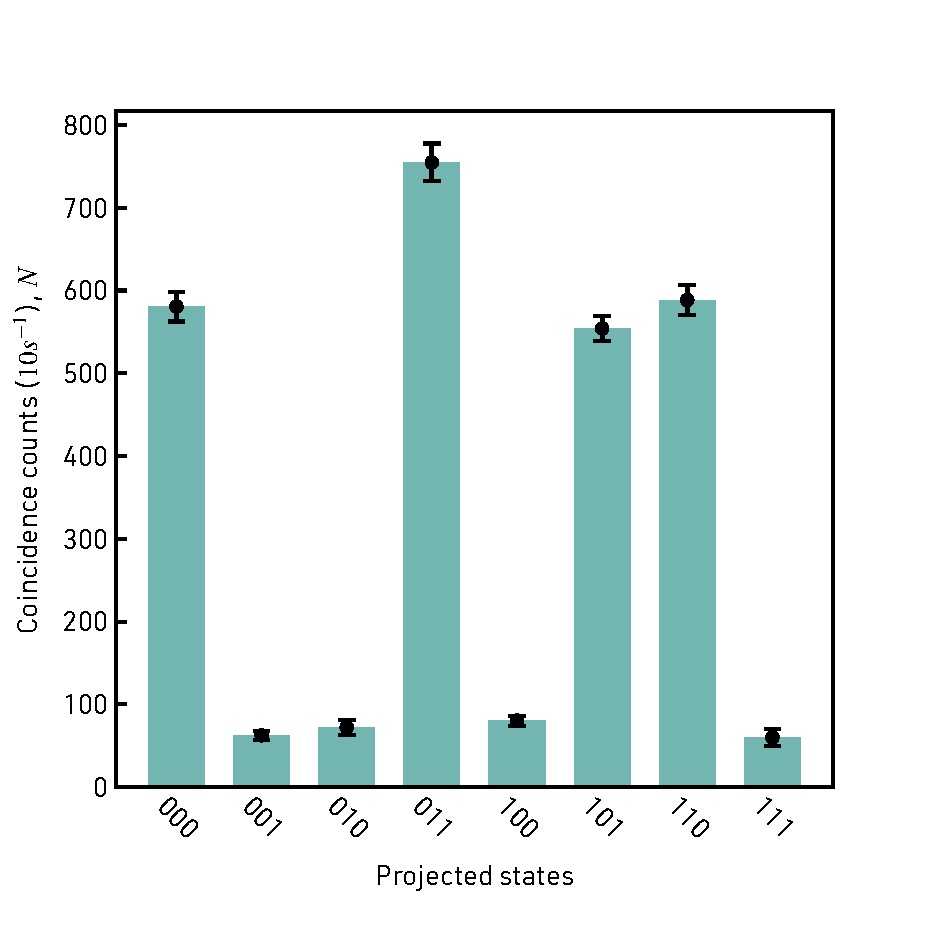
\includegraphics[width=0.33\textwidth]{XYY.pdf}
	}
	\subfloat[\labelFigure{yxy}]
	{
        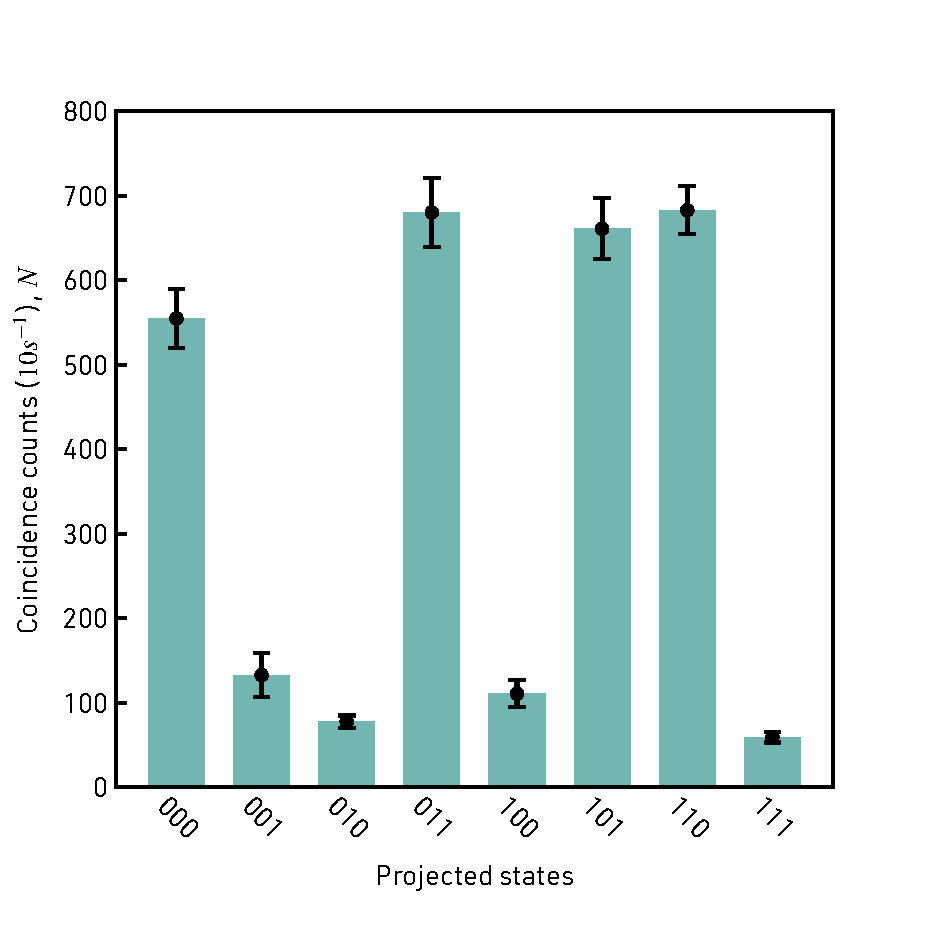
\includegraphics[width=0.33\textwidth]{YXY.pdf}
	} \\
	\subfloat[\labelFigure{yyx}]
	{
        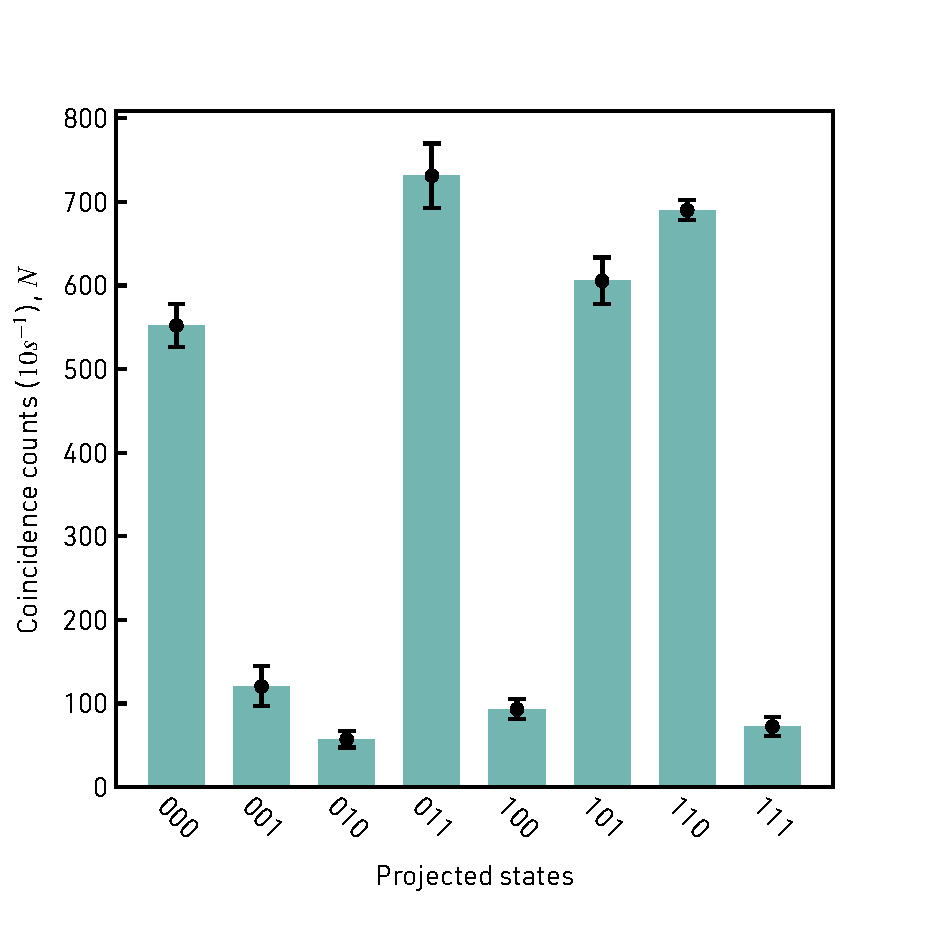
\includegraphics[width=0.33\textwidth]{YYX.pdf}
	}
	\subfloat[\labelFigure{zzz}]
	{
        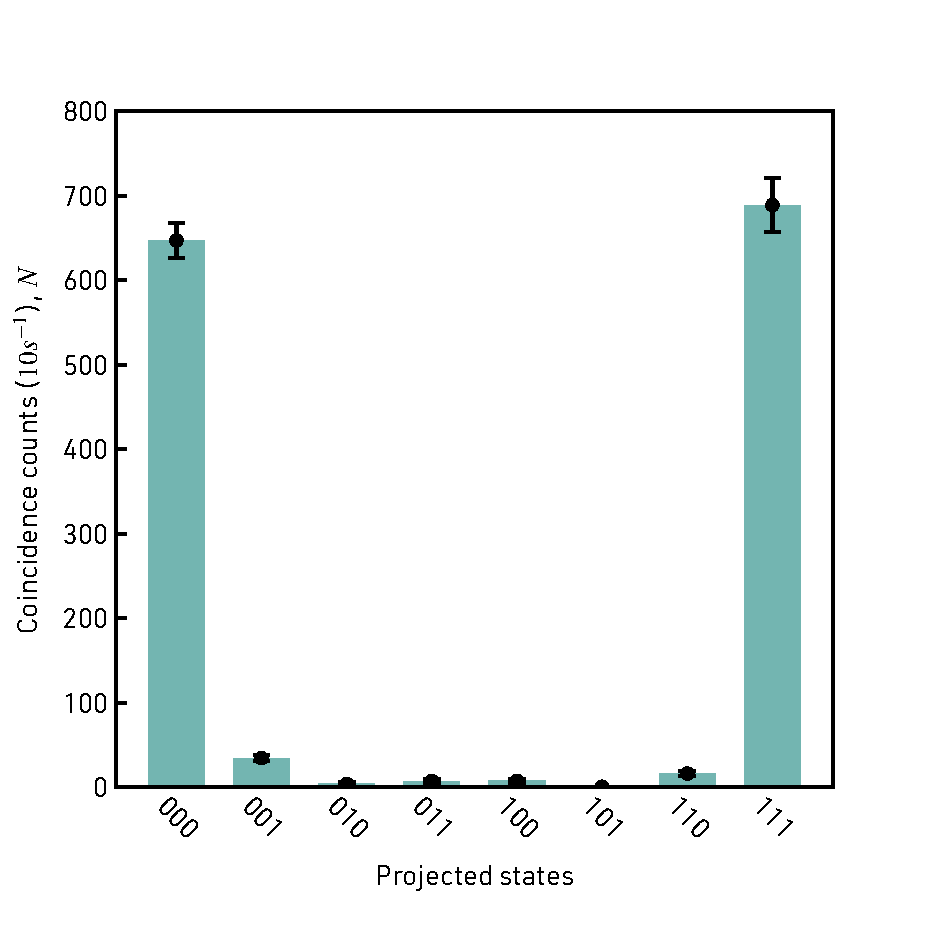
\includegraphics[width=0.33\textwidth]{ZZZ.pdf}
	}
	\caption[Photon coincidence counts of various projected states][-135pt]{Photon coincidence counts of various projected states for the evaluation of the expectation values \textbf{(a)} $\expval{X_1X_2X_3}$ \textbf{(b)} $\expval{X_1Y_2Y_3}$ \textbf{(c)} $\expval{Y_1X_2Y_3}$ \textbf{(d)} $\expval{Y_1Y_2X_3}$ \textbf{(e)} $\expval{Z_1Z_2Z_3}$. The outcomes $0$ and $1$ correspond to the measurement of the positive- and negative-valued eigenvalue of the corresponding Pauli operator, respectively. The error bars represent $95\%$ confidence intervals around the mean value (see section~\protect\refSectionOnly{error_bars} of technical~\protect\refAppendixOnly{appendix_A}).}
	\labelFigure{expvals}
\end{figure*}

\bigskip

\begin{table}[h!]
	\centering
	\caption[Three-qubit operator expectation values for the evaluation of the fidelity and witness of the generated state][20pt]{Three-qubit operator expectation values for the evaluation of the fidelity and witness of the measured state. The values in parenthesis represent $95\%$ confidence intervals around the mean value and derived from the values in ~\protect\refTableOnly{expvals} with appropriate error propagation.}
	\labelTable{expvals}
	\begin{tabular}{ll}
		\toprule
		Operator & Expectation value \\
		\toprule
		$Z_1Z_2Z_3$ & $-0.0453(0.0329)$ \\
		$\mathds{1}_1Z_2Z_3$  & $0.922(0.0329)$\\
		$Z_1\mathds{1}_2Z_3$  & $0.908(0.0329)$\\
		$Z_1Z_2\mathds{1}_3$  & $0.973(0.0329)$\\
		$X_1X_2X_3$ & $-0.807(0.0275)$ \\
		$X_1Y_2Y_3$ & $0.800(0.0163)$ \\
		$Y_1Y_2X_3$ & $0.765(0.0237)$ \\
		$Y_1X_2Y_3$ & $0.743(0.0286)$ \\
		$\mathds{1}_1\mathds{1}_2\mathds{1}_3$ & $1.00(0.0264)$ \\
		\toprule
	\end{tabular}
\end{table}

\bigskip
\noindent
The Bell-Mermin operator (See section~\refSectionOnly{quantum_non_separability}) takes the form:

\begin{align}
	\labelEquation{bell_mermin_3}
	\mathcal{M} = X_1X_2X_3 - X_1Y_2Y_3 - Y_1X_2Y_3 - Y_1Y_2X_3.
\end{align}

\noindent
We can evaluate the expectation value of Bell-Mermin from the same expectation values in~\refTableOnly{expvals}. Our generated state gives a expectation value of $\expval{\mathcal{M}} = 3.137\pm0.0490$, clearly violating the bound of $\ev{\mathcal{M}} = 2$ under the assumption of local realism~\footnote{For the case of a state locally equivalent to a \acs{GHZ} state as in~\refEquationOnly{standard_ghz}, the Bell-Mermin for this state is $\mathcal{M} = -X_1X_2X_3 + X_1Y_2Y_3 + Y_1X_2Y_3 + Y_1Y_2X_3$.}.

\clearpage
\noindent
Lastly, we may further detect the genuine multi-particle entanglement around the expected state (\acs{GHZ}) by means of a stabilizer-based entanglement witness operator $\mathcal{W}$. An stabilizer-based entanglement witness operator for a three-qubit \acs{GHZ} state in its standard form is given by:~\cite{Toth_2005}:
 
\begin{align}
	\mathcal{W} = \frac{3}{2}\mathds{1}_1\mathds{1}_2\mathds{1}_3 - X_1X_2X_3 - \frac{1}{2}\left(Z_1Z_2\mathds{1}_3 + \mathds{1}_1Z_2Z_3 + Z_1\mathds{1}_2 Z_3\right).
\end{align}

\noindent
The above entanglement witness operator has an expectation value of $-1$ with respect to an ideal three-qubit \acs{GHZ} state, since the \acs{GHZ} state has an expectation value of $+1$ with respect to the individual stabilizing operator terms\footnote[][-15pt]{The vigilant reader may notice that Bell-Mermin operator of~\refEquationOnly{bell_mermin_3} resembles a entanglement witness. In fact, it is a disguised entanglement witness for genuine three-qubit entanglement. See Toth~\etal~\cite{Toth_2005}.}. An entanglement witness operator detecting genuine multi-partite entanglement around the ideal state $\ket{\psi}$ has a noise threshold $p_\text{limit}$, that is, it will detect a mixed state of the form $\varrho(p_\text{noise}) = \mathds{1}/2^N + (1- p_\text{noise})\op{\psi}$ as genuinely entangled if $p_\text{noise}$ is below the positive-valued threshold $0<p_\text{limit}<1$~\cite{Toth_2005}; for the above witness $p_\text{limit}=2/5$. 

\bigskip
\noindent
We evaluate the witness for our experimentally generated state~\footnote[][15pt]{For the three-qubit state in~\refEquationOnly{standard_ghz} is a locally equivalent to the three-qubit standard \acs{GHZ} state, its entanglement witness operator is given by $\mathcal{W}=3/2 \mathds{1}_1\mathds{1}_2\mathds{1}_3 + X_1X_2X_3 - \frac{1}{2}\left(Z_1Z_2\mathds{1}_3 + \mathds{1}_1Z_2Z_3 + Z_1\mathds{1}_2 Z_3\right)
$.} using the expectation values of the stabilizing operators in~\refTableOnly{expvals}, we obtain a value of $\Tr(\mathcal{W}\varrho) = -0.709\pm0.0560$, confirming that the generated state exhibits genuine three-qubit entanglement. Furthermore, the expectation value of the above entanglement witness gives a lower bound for the fidelity of the measured state $\varsigma$ with respect to the expected state $\varrho$~\cite{Toth_2005}:

\begin{align}
	F(\varrho, \varsigma) = \Tr(\varrho\varsigma) \geq \frac{1}{2}\left(1 - \expval{\mathcal{W}}\right).
\end{align}

\noindent
As a check for self-consistency, we evaluate the above expression for our experimentally generated state $\varsigma$ and obtain a lower bound of $F(\varrho, \varsigma) \geq 0.854\pm0.0280$, which indeed corroborates our measured fidelity from earlier. 


\bigskip
\noindent
In comparison to similar experiments, particularly that in reference~\cite{Lu_2007} where the generation of a three-qubit three-photon \acs{GHZ} state played a crucial role in an experimental demonstration of Shor's algorithm for the factorization of $15$, they achieve a lower fidelity of $F_\varrho= 0.74 \pm 0.02$. Although their full joint state is product state of a \acs{GHZ} state and $\ket{0}$ (ideally), nonetheless our fidelity results are suggestive of an improvement. Similar reasoning from the previous section may explain the less-than-unity fidelity of our generated state, since this experiment builds upon on it; an improvement of the former will likely improve the latter. Nonetheless, the deviation between the two fidelities is not too great, and the latter result demonstrates that the experimental scheme of Park~\etal~\cite{Park_2007} works well enough in practice, while crucially avoiding the added complications of using two or more \acs{SPDC} processes to generate moderate hyper(hypo)entangled photonic states.

\bigskip
\noindent
As noted earlier, a three-qubit \acs{GHZ} state is locally equivalent to a three-qubit graph state of the form:
\begin{align}
	\labelEquation{c_3}
	\ket{\mathcal{G}_3} = \frac{\ket{+, 0, +} + \ket{-, 1, -}}{\sqrt{2}},
\end{align}

\noindent
which in the circuit model may be generated by an application of controlled-$Z$ (two-qubit gate) operations on neighboring qubits ($1$-$2$ and $2$-$3$) of the initial resource state $\ket{+}_1\ket{+}_2\ket{+}_3$. 


\clearpage
\noindent
Interestingly enough, through only the application of local operators (single-qubit gates) we can generate another graph state, that can be otherwise generated from an application of controlled-$Z$ (two-qubit gate) operations on all neighboring qubits ($1$-$2$ and $2$-$3$, and $1$-$3$) of the initial resource state $\ket{+}_1\ket{+}_2\ket{+}_3$:

\begin{align}
	\labelEquation{c_prime_3}
	\ket{\mathcal{C}'_3} &= \frac{\ket{0, 0, +} + \ket{1,0,-} + \ket{0,1,-} - \ket{1,1,+}}{2}, \nonumber \\
						 &= \frac{\ket{\Phi^-, +}  + \ket{\Psi^+, -}}{\sqrt{2}},
\end{align}

\begin{marginfigure}
    \tikzfig{graphics/GHZ}
    \caption[\acs{LU} equivalent graph states through a single application of the \acs{ELC} rule.]{\acs{LU} equivalent graph states through a single application of the \acs{ELC} rule. A graph state generated with two non-local controlled-$Z$ operations between $1$-$2$ and $2$-$3$ is locally equivalent to a graph state generated with three non-local controlled-$Z$ operations between $1$-$2$, $2$-$3$ and $1$-$3$. The action of an \acs{LU} operation $U_a(G)$ on the level of the graph, for the chosen vertex $a$ (indicated with a dashed outline) an edge is created between its neighbors (opaque indigo line).}
	\labelFigure{ghz_lu_eq}
\end{marginfigure}

\noindent
where $\ket{\Phi^-}$ and $\ket{\Psi^+}$ are two of the Bell states. Thus our experimentally realized state, generated with two non-local gates in the circuit model, is locally equivalent to a graph state, generated with three non-local gates! (See~\refFigureOnly{ghz_lu_eq} for illustration)! A projection of the third qubit (polarization) in either $\ket{+}$ or $\ket{-}$ leaves the qubit $1$ (polarization) and qubit $2$ (path) in the state $\ket{\Phi^-}$ or $\ket{\Psi^+}$, respectively. graph states with this peculiar property are said to belong to same \acs{LU}-equivalence class~\cite{Hein_2004, Nest_2004}.


\bigskip
\noindent
The local unitaries, which may absorbed into our measurement basis, relating the graph state in~\refEquationOnly{c_3} and~\refEquationOnly{c_prime_3} are given by:

\begin{align}
	U = \sqrt{(iZ_1)}\sqrt{(-iX_2)}\sqrt{(iZ_3)}.
	\labelEquation{lu}
\end{align}

\noindent
The experimental components that are used in performing the measurements (translation stages and wave plates), had their operations made fully automatic. Thorlabs provides a host-controller communications protocol, which provides a more fine-grained control over their motorized components. Through the programmatic use of this protocol, the operation of each of the aforesaid motorized components was modularized and made accessible through an application programming interface (API), remotely served by a Raspberry Pi 4. Additionally, we designed a simple mobile graphical user interface (GUI) for this API that gives users~\footnote{At the moment, only the author has access. I will be taking applications for early stage access soon :).} the ability to remotely perform the same data acquisition experiments in this chapter\footnote{Measurements for witness, fidelity, Bell-Mermin inequality violation, etc}. A more-detailed explanation of how this was achieved is of very little scientific interest, and thus can be found in the technical ~\refAppendixOnly{appendix_D}. ~\refFigureOnly{flowchart} shows a schematic flow diagram of the various components as described above, and~\refFigureOnly{demo} shows various demonstrations of the mobile \acs{GUI}. See~\refAppendixOnly{appendix_D} for details.

\begin{figure}[h]
	\centering
	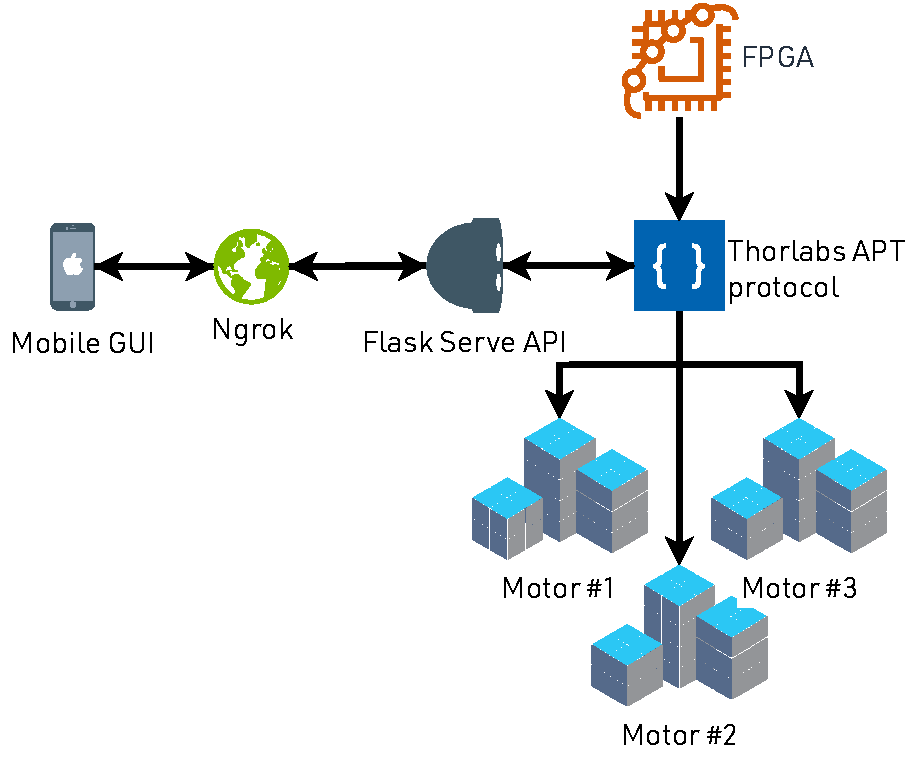
\includegraphics[width=0.7\textwidth]{flowchart}
	\caption[Schematic flow diagram showing the various components.]{Schematic flow diagram showing the various components. Through the \acs{GUI} one can queue up an experiment through an ngrok endpoint, which serves our locally hosted API on a Raspberry Pi served by a Flask server. Depending on the invoked endpoint, the API using invokes APT protocol to trigger the various motors. In the instance, we invoked endpoint is a move; after this execution, an \acs{FPGA} collects the coincidence counts from the single photon detectors and sends them back to the mobile \acs{GUI}.}
	\labelFigure{flowchart}
\end{figure}

\clearpage

\begin{figure}
	\subfloat[]
	{
		\fbox{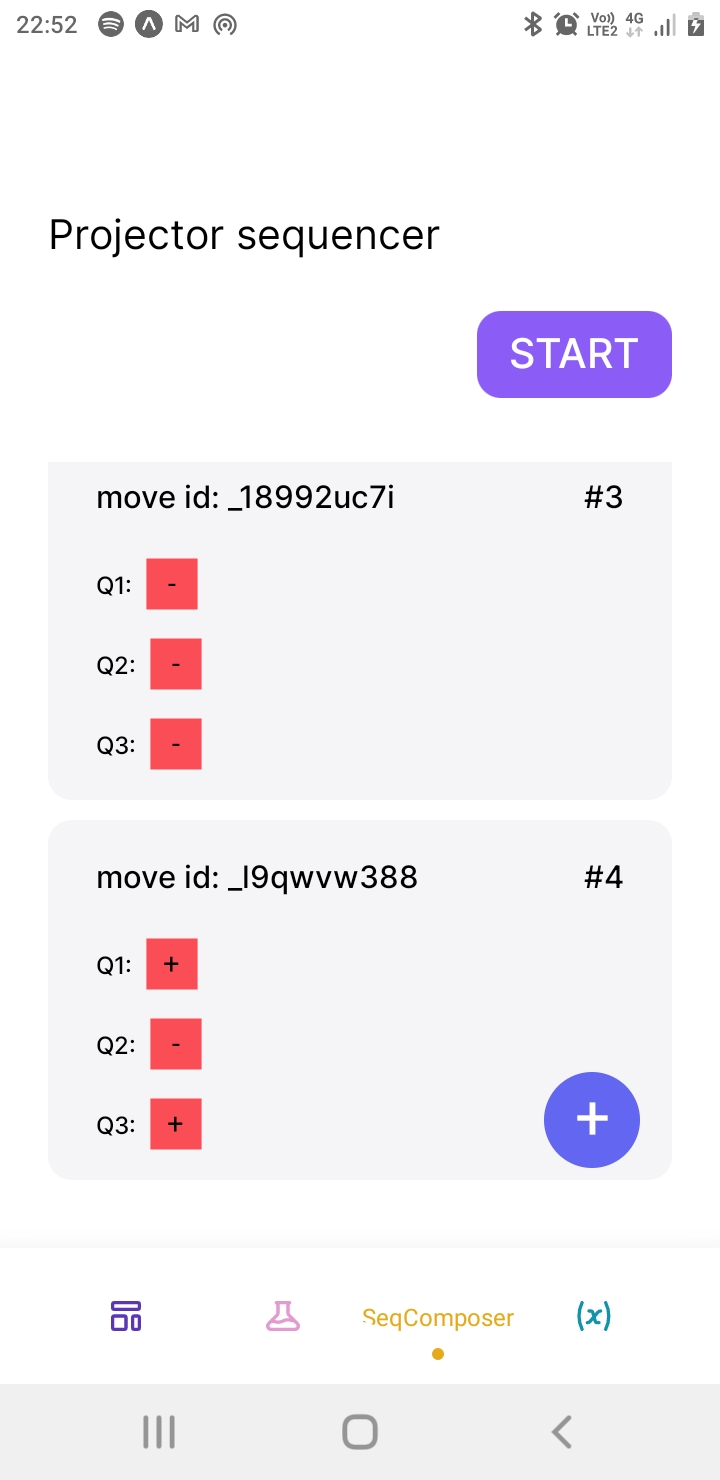
\includegraphics[width=50mm,keepaspectratio]{sequencer4}
	}}
	\subfloat[]
	{
		\fbox{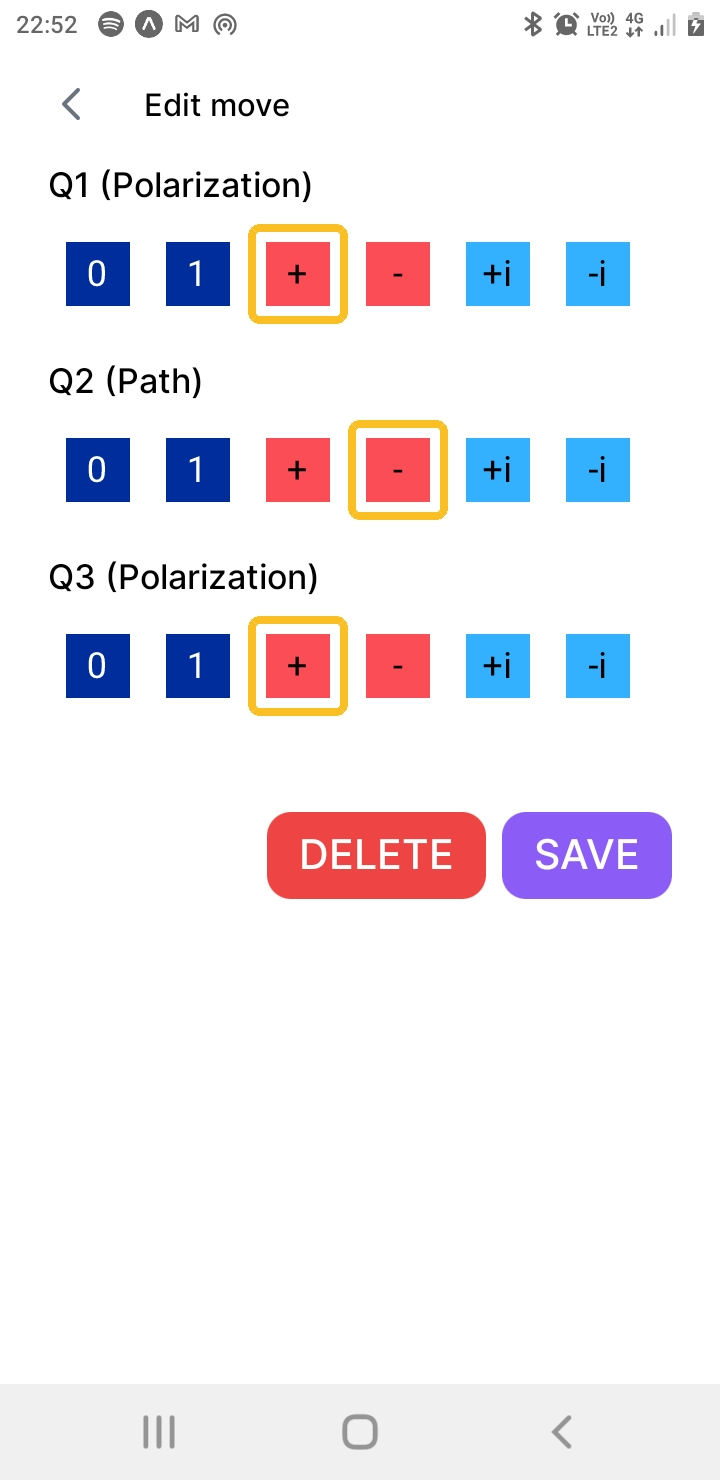
\includegraphics[width=50mm, keepaspectratio]{edit_measurement}
	}} \\
	\subfloat[]
	{
		\fbox{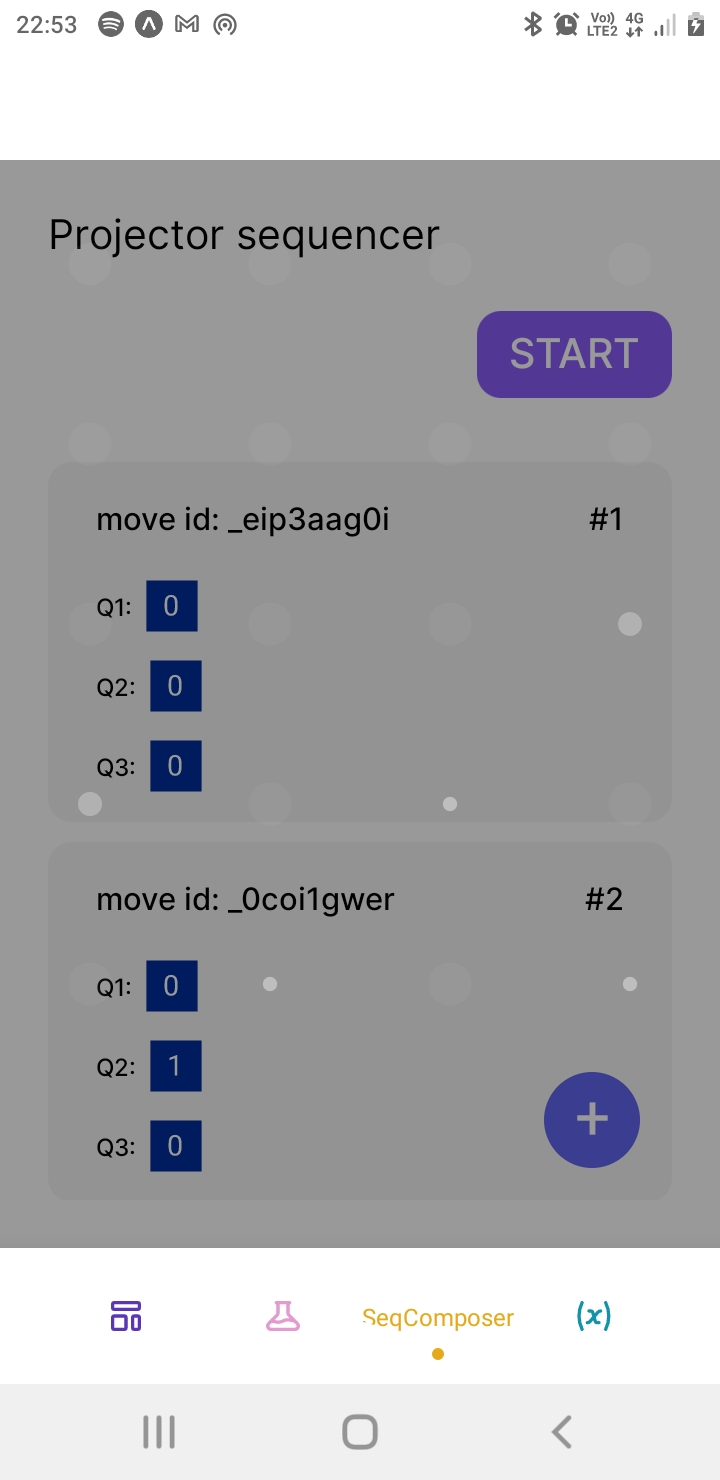
\includegraphics[width=50mm,keepaspectratio]{loading_state}
	}}
	\subfloat[]
	{
		\fbox{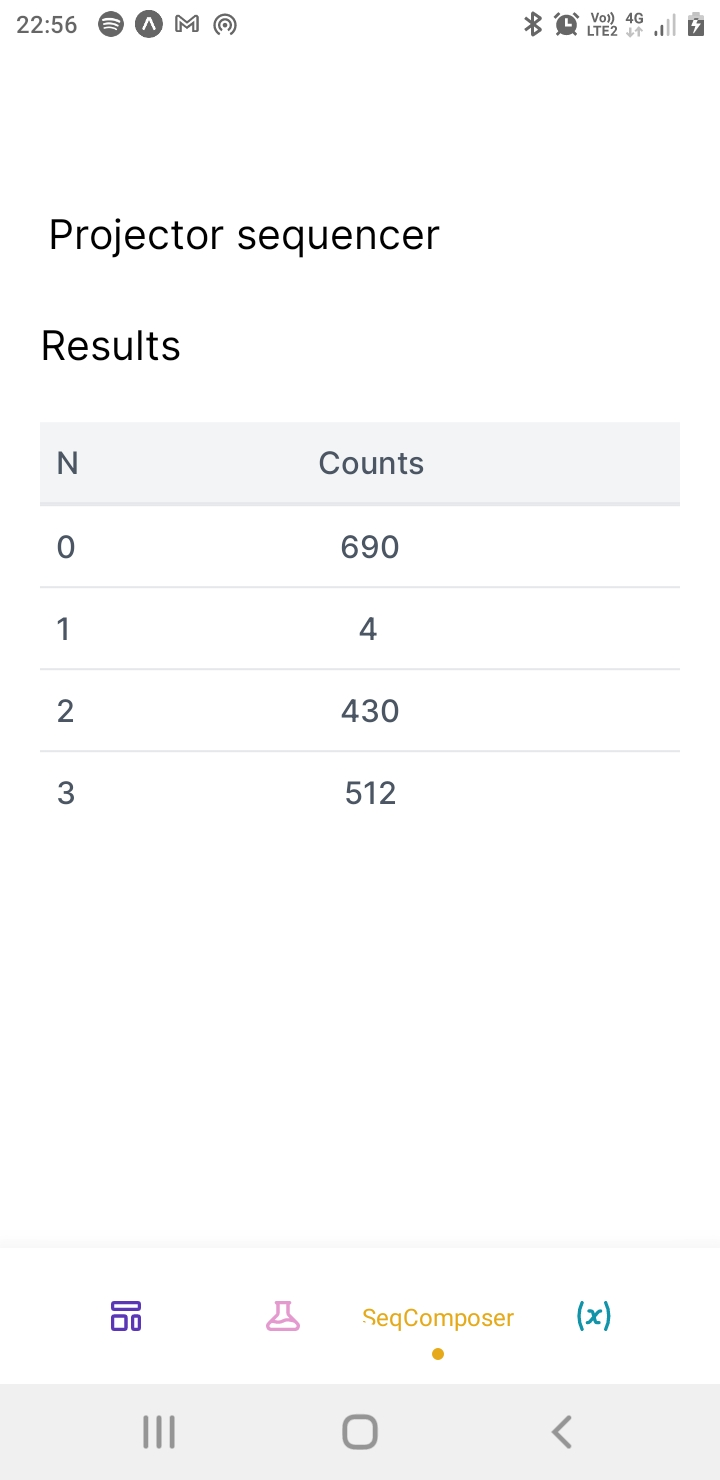
\includegraphics[width=50mm, keepaspectratio]{sequencer_results}
	}} 
	\caption[Various demo screen for the mobile \acs{GUI}.][6pt]{Various demo screens for the mobile \acs{GUI}. See~\protect\refAppendixOnly{appendix_D} for details}
	\labelFigure{demo}
\end{figure}

\clearpage

\section{Concluding remarks}
In this chapter, we described an experimental scheme due to Park~\etal\cite{Park_2007} for generating a two-photon three-qubit polarization-path-entangled \acs{GHZ} state from a Bell-state photon pair source. We experimentally realized this scheme, generating a moderate fidelity state, higher than a previous similar experiment, that is locally equivalent to a three-qubit \acs{GHZ} state and two graph states. Each of the qubits is addressable by measurement, with the path qubit limited to equatorial basis measurements. We also showed that the generated state possess non-local correlations by showing that it leads to a clear violation of the Bell-Mermin inequality. Furthermore, we verify that the non-local correlations the state possesses are indeed due to genuine three-qubit entanglement, by evaluating an entanglement witness for the generated state. Finally, we proceed to make this entanglement source remotely accessible and designed a simple GUI that allows users the ability to perform data acquisition experiments. A possible avenue of departure from here, would be to extend the three-qubit state to a four-qubit state by similarly encoding a path qubit on the other down-conversion photon, which would realize a four-qubit linear graph state, providing an even more versatile $4$-qubit processor on which one can carry out quantum algorithms~\cite{Chen_2007} and other types of quantum protocols, such as quantum games~\cite{Schmid_2010}.


% \begin{marginfigure}
% 	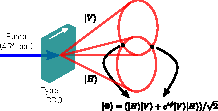
\includegraphics[width=\linewidth]{type-II-SPDC.pdf}
% 	\caption[Two Type-I phase matching]{Type-II phase matching}
% \end{m
